\documentclass{standalone}
\usepackage{tikz}
\usepackage{pgfplots}
\pgfplotsset{compat=newest}
\usetikzlibrary{calc}
\usepackage{ifthen}
\newcommand\mycolor{white}
\usetikzlibrary{matrix}

\begin{document}
    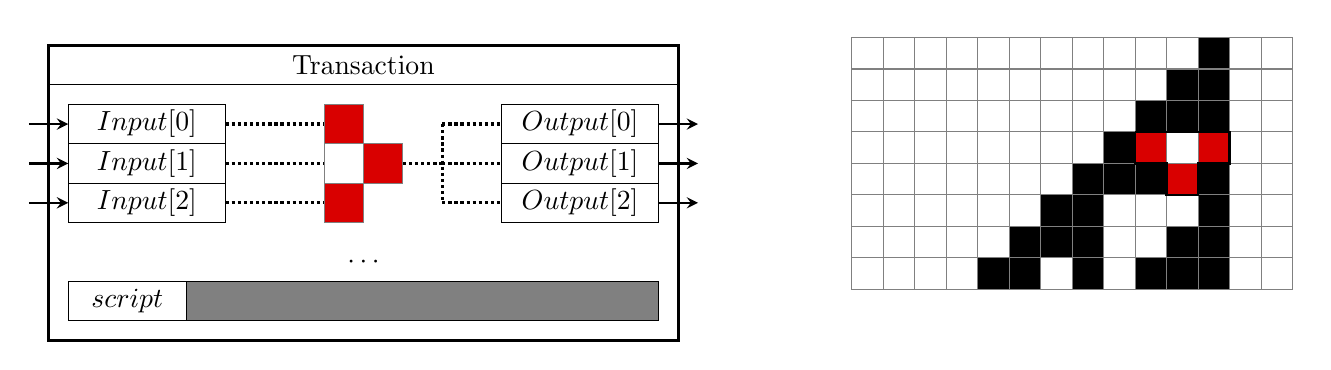
\begin{tikzpicture}[
        X/.style={draw=gray, minimum size=4mm, outer sep=0pt},
        B/.style={X, fill},
        C/.style={X, fill=black!15!red},
        D/.style={X, fill=black!15!red},
        E/.style={X, fill=black!15!red},
        mymatrix/.style={matrix of nodes, row
            sep=-\pgflinewidth,
            column sep=-\pgflinewidth, nodes={X}, nodes in
        empty cells}
    ]

    \def\h{0.5}
    \def\x{8}
    \def\y{3}
    \draw[very thick] (0,0.5*\y) rectangle (\x,{-0.5*(\y-\h)-2*\h});
    \draw (0,0.5*\y-\h) -- node[above,midway] {Transaction} (\x,0.5*\y-\h);

    \foreach \i in {0,1,2}{
        \draw (0.5*\h, {(1.5-\i)*\h}) rectangle  (4.5*\h, {(0.5-\i)*\h}); 
        \node (in1) at (2.5*\h,{(1-\i)*\h}) {$Input[\i]$};
        \draw (\x-0.5*\h, {(1.5-\i)*\h}) rectangle  (\x-4.5*\h, {(0.5-\i)*\h}); 
        \node at (\x-2.5*\h,{(1-\i)*\h}) {$Output[\i]$};
        \draw[thick, ->, >=stealth] (-0.5*\h, {(1-\i)*\h}) -- (0.5*\h, {(1-\i)*\h});
        \draw[thick, ->, >=stealth] (\x-0.5*\h, {(1-\i)*\h}) -- (\x+0.5*\h, {(1-\i)*\h});
        \draw[densely dotted, very thick] (4.5*\h, {(1-\i)*\h}) -- (0.5*\x-\h, {(1-\i)*\h});
        \draw[densely dotted, very thick] (0.5*\x + 2*\h, {(1-\i)*\h}) -- (\x-4.5*\h, {(1-\i)*\h});
    }
    \draw[densely dotted, very thick] (0.5*\x + \h, 0) -- (0.5*\x+2*\h, 0);
    \draw[densely dotted, very thick] (0.5*\x + 2*\h, \h) -- (0.5*\x+2*\h, -\h);

    \draw[C] (0.5*\x - \h, 1.5*\h) rectangle (0.5*\x, 0.5*\h); 
    \draw[X] (0.5*\x - \h, 0.5*\h) rectangle (0.5*\x, -0.5*\h); 
    \draw[C] (0.5*\x - \h, -0.5*\h) rectangle (0.5*\x, -1.5*\h); 
    \draw[C] (0.5*\x , 0.5*\h) rectangle (0.5*\x + \h, -0.5*\h); 

    \draw (0.5*\h, -3*\h) rectangle (\x-0.5*\h, -4*\h);
    \draw[fill=gray] (3.5*\h, -3*\h) rectangle (\x-0.5*\h, -4*\h);
    \node at (2*\h, -3.5*\h) {$script$};
    \node at (0.5*\x, -2.5*\h) {$\cdots$};


    \matrix at (13,0) [mymatrix]{
        &&&&&&&&&&&|[B]|&&\\
        &&&&&&&&&&|[B]|&|[B]|&&\\
        &&&&&&&&&|[B]|&|[B]|&|[B]|&&\\
        &&&&&&&&|[B]|&|[C]|&&|[C]|&&\\
        &&&&&&&|[B]|&|[B]|&|[B]|&|[D]|&|[B]|&&\\
        &&&&&&|[B]|&|[B]|&&&&|[B]|&&\\
        &&&&&|[B]|&|[B]|&|[B]|&&&|[B]|&|[B]|&&\\
        &&&&|[B]|&|[B]|&&|[B]|&&|[B]|&|[B]|&|[B]|&&\\
    };
    \draw[thick] (13.8,0.4) -- (15,0.4) -- (15,0)
    -- (14.6,0) -- (14.6,-0.4) -- (14.2,-0.4) -- (14.2, 0) -- (13.8, 0)
    -- (13.8, 0.4);
    \end{tikzpicture}
\end{document}
